% UniSafe Skills — 课程小组报告
% 编译：XeLaTeX（ctexart 中文支持）。图位于 ./figures/（与本文件同目录）。
% 数据来源：report_artifacts/result_summary.csv（复算，与各 metrics.md 逐位一致）；不含虚构数字。
% 注意：第 2 节（方向 A 数据集）留给甲撰写，乙不代写。
\documentclass[11pt]{ctexart}
\usepackage[a4paper,margin=2.4cm]{geometry}
\usepackage{graphicx}
\usepackage{booktabs}
\usepackage{float}
\usepackage{caption}
\usepackage{amsmath}
\usepackage{xcolor}
\usepackage[hidelinks]{hyperref}
\graphicspath{{figures/}}
\captionsetup{font=small,labelfont=bf}
\setlength{\parskip}{0.4em}

\title{\textbf{UniSafe Skills：统一 Schema 下的跨模态内容安全 Guard 评测}\\
\large 方向 A（Dataset Skill）+ 方向 B（Guard Skill）配套实验平台}
\author{[学生甲（方向 A）] \quad [学生乙（方向 B）]} % TODO: 填真实姓名/学号
\date{2026-06-17}

\begin{document}
\maketitle

\begin{abstract}
\noindent
本报告构建了一个以统一 JSONL schema 与统一 Guard 结果接口为核心的内容安全评测平台：方向 A 将三个安全数据集（文本 WildGuardMix + XSTest 过度拒答探针、图像 UnsafeBench）规整为同一格式，方向 B 用同一套 Guard 接口跨文本/图像模态封装多种 guard 并评测。文本侧 Llama Guard 3 在 1{,}959 条真实测试集上取得 AUROC~0.888、过度拒答率 6.4\%，表现稳健；图像侧 ShieldGemma~2（int8）受三策略覆盖与 19.4\% 的量化 NaN 限制，AUROC 仅 0.613（CPU bf16 真值 0.719）。我们以\textbf{双口径指标}（answered\_only / failure\_as\_wrong）防止"剔除失败样本导致虚高"，以\textbf{阈值校准}（而非 ensemble）作为效果杠杆，并以\textbf{逐记录 NaN 回退（E3）}把图像侧覆盖率从 80.6\% 补回至投影 $\sim$100\%。全部结果数字均由保存的预测复算、与权威 \texttt{metrics.md} 逐位一致，并对三类结构上限（三策略天花板、判官对抗坍塌、int8 量化漂移）如实定位、不声称解决。\\[0.4em]
\noindent\textbf{关键词}：内容安全 Guard；统一 schema；Llama Guard；ShieldGemma 2；双口径评测；阈值校准；可复现性。\\
\noindent\textbf{Keywords}: content-safety guard; unified schema; Llama Guard; ShieldGemma 2; dual-basis evaluation; threshold calibration; reproducibility.
\end{abstract}

\section{引言（项目概述）}
本作业要求两人一组、以\textbf{流水线}方式协作：方向 A 产出"内容安全数据集 $\to$ 统一 JSONL"的 Dataset Skill，方向 B 产出"封装 Guard 模型/规则/API $\to$ 统一安全判断"的 Guard Skill，且方向 B 必须在方向 A 构造的数据集上完成评测。我们锁定的统一叙事是：\emph{同一套 unified schema 与同一个 Guard 结果接口，跨文本与图像模态泛化}——这直接回应作业"统一实验平台"的目标。

方案采用"文本核心 + 多模态亮点"：文本侧做扎实、先过格式校验再出指标，图像侧严格限定小样本以保护可复现性。分工上，甲负责两个 dataset skill（\texttt{dataset-wildguardmix}、\texttt{dataset-unsafebench}），乙负责两个 guard skill（\texttt{guard-llama-guard}、\texttt{guard-shieldgemma2}），贡献约各半。本报告聚焦方向 B 的 guard 方法与联合实验（第 3--6 节）；\textbf{第 2 节（方向 A 数据集）由甲撰写}。全文围绕作业评分三轴展开：结构与功能完整性、可复现性、结果与报告。

\section{数据集构建说明与分析（方向 A）}
\textcolor{gray}{\itshape 【本节留给方向 A 同学（甲）撰写：数据集选型与统一 schema、规模与基准率（含 safe / 安全探针样本对 FPR 与过度拒答率的支撑）、通过 \texttt{dataset-format-checker}（exit 0）的质量门，以及 caption 真数据覆盖等 caveat。乙不代写；写作要点与必读证据见 \texttt{报告大纲.md} 第 1 节与"证据地图"。】}

\section{Guard 方法说明与分析（方向 B）}

\subsection{Guard 矩阵}
\textbf{文本侧}三种 guard 互为对照：(1) \textbf{Llama Guard 3-1B}，本地推理，以 unsafe 词元的归一化概率为连续置信分；(2) \textbf{规则基线}，纯关键词、零依赖，仅给 0/1 判定，因此\emph{无连续分、不计 AUROC}（如实标注，而非缺数据）；(3) \textbf{LLM-as-judge}，调用商用 API，自报置信度经"方向映射"后才参与 AUROC（未映射前实测仅 0.375，跨 guard 的 AUROC 不可直接混比）。\textbf{图像侧}为 (4) \textbf{ShieldGemma~2-4B}，本地 int8 量化，仅 dangerous / sexual / violence 三策略；(5) \textbf{caption-rule}，零依赖的标题/OCR 关键词基线。

\subsection{统一 Guard 结果接口}
五个 guard 共享同一输出 schema、同一退出码契约（0 成功 / 2 部分可用 / 3 致命）、以及"结果分层状态机"（fallback\_only $\to$ partial $\to$ full）。图像 guard 与文本 guard 的输出记录\textbf{零 schema 变更}，使同一套指标机与同一份评测脚本可直接跨模态复用——这是"统一平台"在工程层面的落点。

\subsection{Skill 工程质量}
围绕评分中权重最高的"结构与功能"与"可复现性"，我们落实了若干工程纪律：(a) \textbf{标准 Skill 结构}（\texttt{SKILL.md} + \texttt{scripts/references/schemas/templates/examples/tests}），零安装即可 \texttt{python scripts/main.py} 运行；(b) \textbf{受控复制纪律}：\texttt{validate.py}/\texttt{metrics.py}/\texttt{calibrate.py} 在文本与图像两侧镜像，并以"答案钥双算"锁定一致；(c) \textbf{双口径指标}（见 \S4.3）防止量化失败被静默剔除而虚高；(d) \textbf{优雅降级}：门控模型缺访问时以退出码 2 + 可复制修复提示退出而非崩溃，逐条 try/except 计数，软超时丢弃迟到结果；(e) \textbf{可复现性硬化}：\texttt{run\_metadata} 记录 model\_revision 与库版本、固定随机种子、提供 \texttt{--limit} smoke 路径。

\section{实验流程、结果报告与分析}

\subsection{实验流程}
实验按里程碑推进：M1 打通文本端到端 $\to$ M2 多 Guard 横向对比 + 过度拒答 + 对抗/类别分桶 $\to$ M3 图像多模态亮点 $\to$ M3.5 性能优化 $\to$ M3.6 判别效果优化（阈值校准）$\to$ M3.7 图像覆盖率回退（E3）。全程坚持"先文本扎实、多模态限小样本"，以免拖垮可复现性。本节所有数字取自 \texttt{report\_artifacts/result\_summary.csv}（由保存的逐条预测复算，与权威 \texttt{metrics.md} 逐位一致）。

\subsection{文本侧结果}
表~\ref{tab:text} 给出文本侧三 guard 的 answered\_only 战绩，图~\ref{fig:quality} 直观对比 Accuracy / F1 / Coverage。Llama Guard 综合最强：AUROC~0.888、Accuracy~0.899、Recall~0.660（95\% CI $[0.601,0.715]$）、FPR~0.063，且失败率仅 2.4\%。过度拒答方面，在 250 条 XSTest 安全探针上误报率 6.4\%。对抗鲁棒性可量化：Llama Guard 的 AUROC 从非对抗 0.919 降到对抗 0.831；而 LLM-judge 虽然召回最高（0.750，CI $[0.598,0.858]$），其 FPR 也最高（0.152），且\textbf{对抗下坍塌最严重}（AUROC $0.976 \to 0.633$）——印证"推理判官范式"相对专用 guard 的结构性弱点。我们另实测否定了 ensemble：rule+llama 的 OR/AND 组合无一在 F1 上胜过 Llama Guard 单独，\emph{阈值校准才是真正的效果杠杆}（见 \S4.5）。

\begin{table}[H]
\centering
\caption{文本侧 guard 战绩（answered\_only 口径；正类=unsafe；规则基线无连续分故 AUROC=N/A）。judge 子集为分层 120 条（40 unsafe/40 safe/40 XSTest），基准率与全量 1{,}959 不同，故 Accuracy/FPR 不与全量直接可比，AUROC 更可比。}
\label{tab:text}
\small
\begin{tabular}{lcccccc}
\toprule
guard & $n$ & Acc & Recall & FPR & Macro-F1 & AUROC \\
\midrule
rule & 1959 & 0.798 & 0.271 & 0.112 & 0.582 & N/A \\
\textbf{Llama Guard 3-1B} & 1959 & \textbf{0.899} & 0.660 & 0.063 & \textbf{0.792} & \textbf{0.888} \\
LLM-judge & 120 & 0.815 & \textbf{0.750} & 0.152 & 0.795 & 0.895 \\
\bottomrule
\end{tabular}
\end{table}

\begin{figure}[H]
\centering
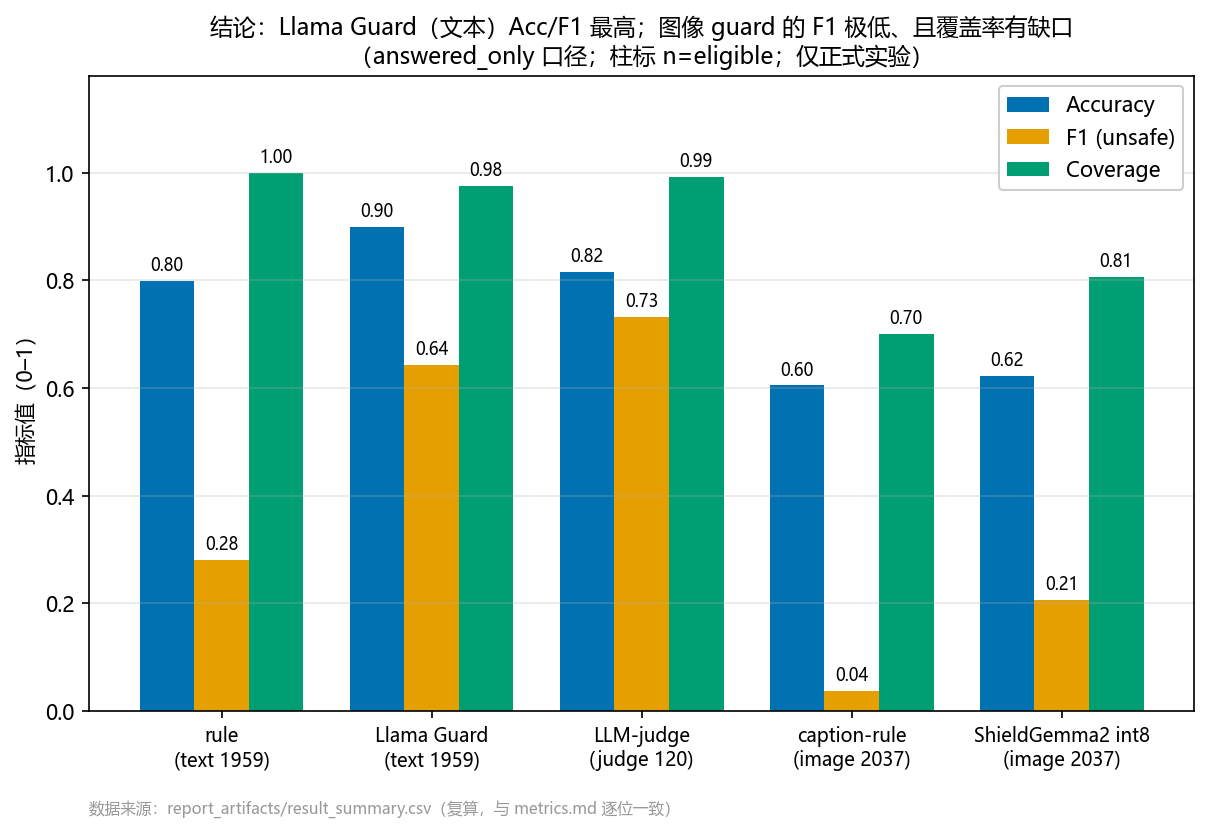
\includegraphics[width=0.82\textwidth]{fig1_guard_quality.png}
\caption{各 guard 的 Accuracy / F1(unsafe) / Coverage（answered\_only）。Llama Guard 文本侧 Acc/F1 最高；图像 guard 的 F1 极低且覆盖率有缺口。柱标 $n=$ eligible。}
\label{fig:quality}
\end{figure}

\subsection{图像侧结果}
图像侧的核心是\textbf{量化与覆盖率的双重制约}（表~\ref{tab:image}，图~\ref{fig:fail}）。ShieldGemma~2 在 int8 下 AUROC 仅 0.613，而同模型 CPU bf16 无量化参考为 0.719——\textbf{0.613 是量化退化下界，不是模型真实水平}，报告须双值并报。失败侧，int8 在自然图像上有 \textbf{19.4\%（395/2037）的确定性 NaN}（同图每次坏成一样），caption-rule 则因真图缺乏描述性标题而近乎失明（Recall~0.020、覆盖率仅 0.701，609 条因缺图/缺 caption 计为 error）。即便用 CPU 真值，ShieldGemma~2 也受\textbf{三策略天花板}限制：UnsafeBench 的 11 个类别里 8 类无对应策略，AUROC 约 0.72 即封顶——属结构上限，非校准/工程可解。

\begin{table}[H]
\centering
\caption{图像侧 guard 战绩（answered\_only）。CPU bf16 为无量化真值参考（非生产精度）；+E3 为对 int8-NaN 子集回退后的恢复子集（见 \S4.6）。}
\label{tab:image}
\small
\begin{tabular}{lccccccc}
\toprule
guard（精度） & $n$ & Acc & Recall & FPR & Macro-F1 & AUROC & Coverage \\
\midrule
caption-rule & 2037 & 0.605 & 0.020 & 0.014 & 0.395 & N/A & 0.701 \\
ShieldGemma2 \textbf{int8}（生产） & 2037 & 0.622 & 0.125 & 0.051 & 0.480 & \textbf{0.613} & 0.806 \\
ShieldGemma2 CPU bf16（参考） & 150 & 0.733 & 0.350 & 0.011 & 0.664 & \textbf{0.719} & 1.000 \\
ShieldGemma2 \textbf{+E3}（NaN 子集） & 100 & 0.790 & 0.393 & 0.056 & 0.689 & 0.675 & 1.000 \\
\bottomrule
\end{tabular}
\end{table}

\begin{figure}[H]
\centering
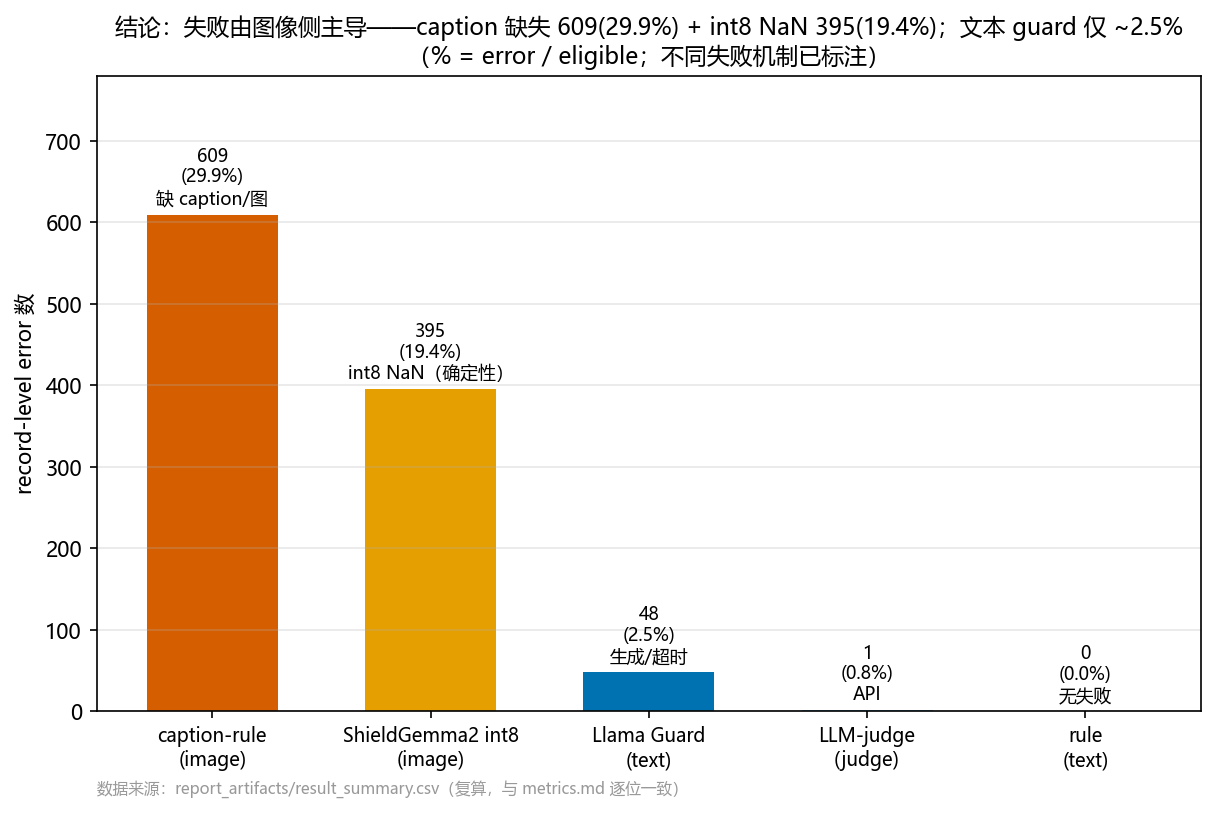
\includegraphics[width=0.80\textwidth]{fig3_failure_types.png}
\caption{record-level 失败的来源与规模。图像侧主导：caption 缺失 609（29.9\%）+ int8 NaN 395（19.4\%）；文本 guard 仅约 2.5\%。}
\label{fig:fail}
\end{figure}

\subsection{双口径指标（防虚高护栏）}
对会失败的 guard，"剔除失败"会让指标偏乐观，"失败计错"会偏悲观，真值落在两者之间——我们因此\textbf{强制并报双口径}（图~\ref{fig:dual}）。落差与失败率成正比：caption-rule 的 Accuracy 从 0.605 降到 0.424（$\Delta-0.18$）、ShieldGemma~2 int8 从 0.622 降到 0.502（$\Delta-0.12$），而文本侧 Llama Guard 仅 $\Delta-0.02$。这张图本身就是"双口径=工程护栏"的活例。

\begin{figure}[H]
\centering
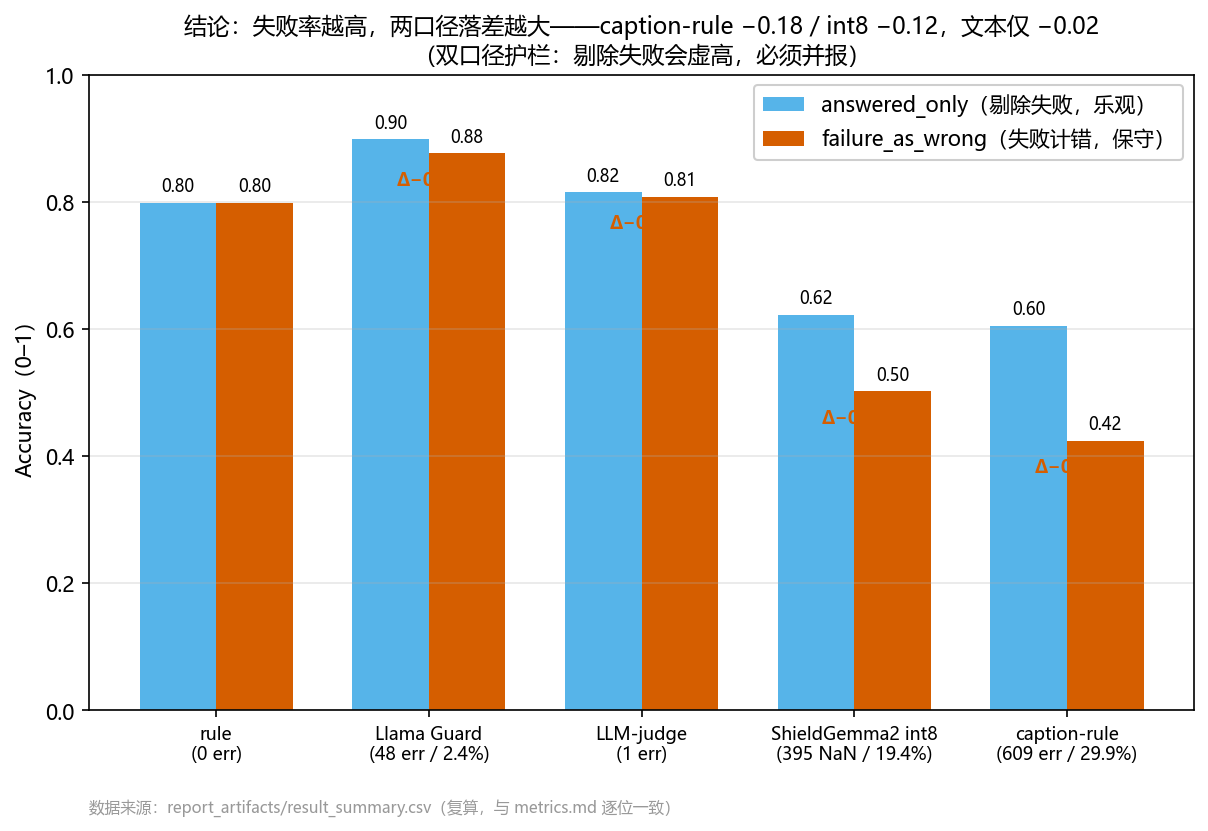
\includegraphics[width=0.80\textwidth]{fig2_dual_basis_gap.png}
\caption{answered\_only 与 failure\_as\_wrong 两口径的 Accuracy 对比。失败率越高，两口径落差越大；剔除失败会虚高，故必须并报。}
\label{fig:dual}
\end{figure}

\subsection{效果优化：before $\to$ after（M3.6 阈值校准）}
我们以 ROC 阈值扫描得到生产阈值并落为默认。Llama Guard 由原生 argmax 调到阈值 0.55：这\textbf{不是 Macro-F1 杠杆而是 precision-favoring 操作点}——对真实旧行为，Macro-F1 几乎持平，真实赢点是 \textbf{FPR $0.063 \to 0.056$、过度拒答 $6.4\% \to 6.0\%$}，代价是召回约降 3\%（如实口径，详见 \texttt{M3.6\_summary.md} \S2.0）。ShieldGemma~2 由 0.5 调到 0.30（取 FPR$\le$0.1 档而非 max\_macro\_f1=0.05/FPR~38\% 的不可接受点）：Macro-F1 $0.480 \to 0.523$、Recall $0.125 \to 0.198$，FPR 仍守 $<0.1$。

\subsection{图像覆盖率回退（M3.7 / E3）}
针对 int8 的 19.4\% NaN，我们实现\textbf{逐记录 NaN 回退}：当 int8 返回 NaN 时，对该单图回退到非量化精度（CPU bf16）重算，默认关闭（\texttt{--nan-fallback none} 复现旧行为）。在 100 张 NaN 子集上\textbf{恢复 100/100}，子集覆盖率 $0\% \to 100\%$、全量覆盖率投影 $80.6\% \to \sim$100\%（图~\ref{fig:cov}）。恢复分是 truth-grade（子集 AUROC~0.675，贴近 CPU 真值 0.719、远高于 int8 下界 0.613）。但必须诚实：\textbf{E3 是覆盖率/鲁棒性赢点，不是 int8 质量修复}——全量在 E3 后为混精度（多数仍是漂移的 int8），且 0.30 阈值在 int8 上校准、套在 bf16 上非最优。

\begin{figure}[H]
\centering
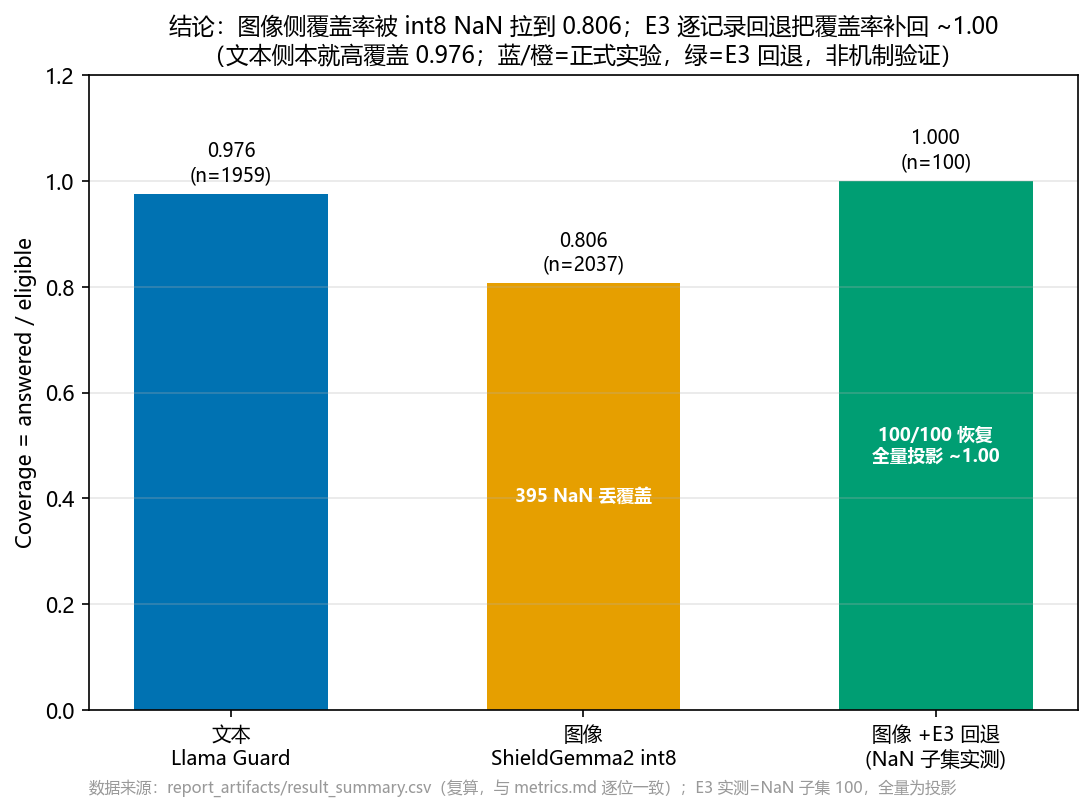
\includegraphics[width=0.72\textwidth]{fig4_completeness_text_vs_image.png}
\caption{文本/图像/图像+E3 的覆盖率对照。图像侧被 int8 NaN 拉到 0.806，E3 逐记录回退补回 $\sim$1.00；文本侧本就高覆盖 0.976。蓝/橙为正式实验，绿为 E3 回退（非机制验证）。}
\label{fig:cov}
\end{figure}

\subsection{性能与可复现性}
M3.5 把 LLM-judge 的并发从串行提到 4 路，实测 $340\text{s} \to 88\text{s}$（\textbf{3.86$\times$}），且逐 id 结果一致；int8 重跑 flip\_rate=0（确定性）。交付前复现核对：两侧单测 \texttt{guard-llama-guard} 105 / \texttt{guard-shieldgemma2} 110 全绿，干净 clone 可离线复现 rule guard 的"预测$\to$评分"全链；真数据级指标的复现需 GPU + HuggingFace 缓存 + 真实数据集（数据/权重按设计不入库，如实定位）。

\subsection{结构上限（未解决，仅定位）}
三类上限属结构性、非本轮校准/工程能解：(1) ShieldGemma~2 \textbf{三策略天花板}（AUROC 即便 CPU 真值也 $\sim$0.72 封顶，需换多策略模型）；(2) \textbf{判官对抗坍塌}（AUROC $0.976 \to 0.633$）；(3) \textbf{int8 量化漂移}（连非-NaN 分也仅约一半可信，E3 只补覆盖、不动质量）。报告对此如实呈现，不声称解决。

\section{结论与局限}
本平台证明了"统一 schema + 统一 Guard 接口跨模态泛化"的可行性：文本侧 Llama Guard 强（AUROC~0.888），工程质量与可复现性扎实，效果以阈值校准而非 ensemble 提升，图像覆盖率以 E3 逐记录回退补回。局限是结构性的——三策略天花板、判官对抗坍塌、int8 量化漂移，E3 只补覆盖、未解此三者。后续方向：换非量化精度以解 int8 漂移、换多策略图像模型以解三策略天花板。

\section{小组成员贡献度}
分工约各半（$\sim$50/50），按 CRediT 角色：\textbf{甲（方向 A）}负责数据获取、统一格式转换、taxonomy 映射与通过 \texttt{dataset-format-checker}（\texttt{dataset-wildguardmix}、\texttt{dataset-unsafebench}）。\textbf{乙（方向 B）}负责 guard 方法封装、统一指标机与双口径实现、阈值校准、性能优化与可复现性硬化、E3 覆盖率回退及结果分析与图表（\texttt{guard-llama-guard}、\texttt{guard-shieldgemma2}）。\textbf{共同}完成 M0 接口契约、22 类 canonical taxonomy 映射与本报告。

\section*{声明}
\textbf{AI 使用}：本项目在编码、结果复算与报告起草中使用了 AI 辅助工具（Claude Code）；所有结果数字均来自本组自有实验、由保存的预测复算并经人工核对，无人工填造。\textbf{数据与代码可得性}：代码与聚合结果见仓库 \href{https://github.com/Lang-Qiu/unisafe-skills}{Lang-Qiu/unisafe-skills}；真实数据集与模型权重依许可与体积不入库（可由 dataset skill 在线重建）。复算与绘图脚本见 \texttt{report\_artifacts/}。

\section*{参考资源}
\small
\begin{itemize}\itemsep0.1em
\item WildGuardMix 数据集（\texttt{allenai/wildguardmix}，odc-by）；XSTest 过度拒答探针（\texttt{walledai/XSTest}）。
\item UnsafeBench 图像数据集（\texttt{yiting/UnsafeBench}）。
\item Llama Guard 3-1B（\texttt{meta-llama/Llama-Guard-3-1B}）；ShieldGemma 2-4B（\texttt{google/shieldgemma-2-4b-it}）。
\item 格式校验器 \texttt{dataset-format-checker}（嵌套 unified schema + 22 类 canonical taxonomy）。
\item 本组实验产物：\texttt{report\_artifacts/result\_summary.csv}、\texttt{analysis\_notes.md}、各 \texttt{M*\_summary.md}、\texttt{REPRODUCTION.md}。
\end{itemize}

\end{document}
